\documentclass[9pt,aspectratio=43,mathserif,table]{beamer} 
%设置为 Beamer 文档类型,设置字体为 10pt,长宽比为16:9,数学字体为 serif 风格
\batchmode

\usepackage{graphicx}
\usepackage{animate}
\usepackage{hyperref}

%导入一些用到的宏包
\usepackage{amsmath,bm,amsfonts,amssymb,enumerate,epsfig,bbm,calc,color,ifthen,capt-of,multimedia,hyperref}
\usepackage{xeCJK} %导入中文包
\setCJKmainfont{SimSun} %字体采用黑体  Microsoft YaHei

% \usetheme{Marburg} %主题
% \usecolortheme{sustech} %主题颜色
\usetheme{metropolis} %主题
% \usetheme{Montpellier}
\usecolortheme{default} %主题颜色

\usepackage[ruled,linesnumbered]{algorithm2e}

\usepackage{fancybox}
\usepackage{xcolor}
\usepackage{times}

\usepackage{listings}

\usepackage{booktabs}
\usepackage{colortbl}

\usepackage{setspace}

% \usepackage{minted}
% \usemintedstyle{emacs}

\newcommand{\Console}{Console}
\lstset{ %
  % backgroundcolor=\color{white},   % choose the background color
  basicstyle=\footnotesize\rmfamily,     % size of fonts used for the code
  columns=fullflexible,
  breaklines=true,                 % automatic line breaking only at whitespace
  captionpos=b,                    % sets the caption-position to bottom
  tabsize=4,
  commentstyle=\color{mygreen},    % comment style
  escapeinside={\%*}{*)},          % if you want to add LaTeX within your code
  keywordstyle=\color{blue},       % keyword style
  stringstyle=\color{mymauve}\ttfamily,     % string literal style
  numbers=left, 
  % numberstyle=\tiny\color{mygray},
  frame=left,
  rulesepcolor=\color{red!20!green!20!blue!20},
  % identifierstyle=\color{red},
  language=c++,
  morekeywords={alignas,continute,friend,register,true,alignof,decltype,goto,
  reinterpret_cast,try,asm,defult,if,return,typedef,auto,delete,inline,short,
  typeid,bool,do,int,signed,typename,break,double,long,sizeof,union,case,
  dynamic_cast,mutable,static,unsigned,catch,else,namespace,static_assert,using,
  char,enum,new,static_cast,virtual,char16_t,char32_t,explict,noexcept,struct,
  void,export,nullptr,switch,volatile,class,extern,operator,template,wchar_t,
  const,false,private,this,while,constexpr,float,protected,thread_local,
  const_cast,for,public,throw,std},
  emph={map,set,multimap,multiset,unordered_map,unordered_set,
    unordered_multiset,unordered_multimap,vector,string,list,deque,
    array,stack,forwared_list,iostream,memory,shared_ptr,unique_ptr,
    random,bitset,ostream,istream,cout,cin,endl,move,default_random_engine,
    uniform_int_distribution,iterator,algorithm,functional,bing,numeric}
}


\setsansfont{Consolas}
\setmainfont{SimSun}

\definecolor{mygreen}{rgb}{0,0.6,0}
\definecolor{mymauve}{rgb}{0.58,0,0.82}
\definecolor{mygray}{gray}{.9}
\definecolor{mypink}{rgb}{.99,.91,.95}
\definecolor{mycyan}{cmyk}{.3,0,0,0}


%题目,作者,学校,日期
\title{\fontsize{14pt}{14pt} Title}
\subtitle{\fontsize{11pt}{14pt}\textbf{Subtitle}}
\author{\fontsize{8pt}{14pt}Author}  % If in Chinese, change 8pt to 10pt
\institute{\fontsize{8pt}{14pt} Computer Science Institute}
\date{\today}

% %学校Logo
% \pgfdeclareimage[height=1.5cm]{nudt-logo}{figures/nudt.png}
% \logo{\pgfuseimage{nudt-logo}\hspace*{0.1cm}\vspace*{-1cm}}


% \AtBeginSection[]
% {
%   \begin{frame}<beamer>
%   \begin{spacing}{0.5}
%     \frametitle{\textbf{Table of Contents}}\small
%     \tableofcontents[currentsection]
%   \end{spacing}
% \end{frame}
% }
\AtBeginSubsection[]
{
  \begin{frame}<beamer>
  \begin{spacing}{0.5}
    \frametitle{\textbf{Table of Contents}}\small
    \tableofcontents[currentsection, currentsubsection]
  \end{spacing}
\end{frame}
}
\beamerdefaultoverlayspecification{<+->}
% -----------------------------------------------------------------------------
\begin{document}
% -----------------------------------------------------------------------------

\frame{\titlepage}

\section[Table of Contents]{}   %Table of Contents
\begin{frame}{Table of Contents}\small
  \begin{spacing}{0.5}
    \tableofcontents
  \end{spacing}
\end{frame}

% -----------------------------------------------------------------------------
\section{Section1}  %引言
\subsection{Background Information}
\begin{frame}
  % \frametitle<presentation>{What is DSE \footnotemark[1] \footnotetext[1]{Reference: http://zbchen.github.io/Papers_files/icse2015.pdf}}
  \frametitle<presentation>{framename}
  \begin{columns}[T] % align columns
    \begin{column}<0->{.5\textwidth}
      \begin{itemize}
        \item item1
        \item item2
      \end{itemize}
    \end{column}%
    \hfill%
    \begin{column}<0->{.7\textwidth}
      \begin{figure}[thpb]
        \centering
        \resizebox{1\linewidth}{!}{
          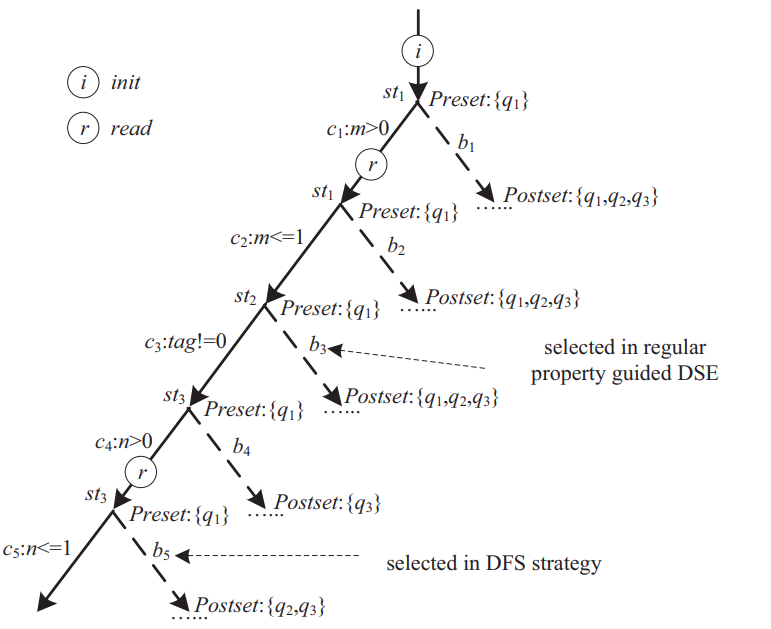
\includegraphics{figures/dse.png}
        }
        %\includegraphics[scale=1.0]{figurefile}
        \caption{DSE}
        \label{fig:dse}
      \end{figure}
    \end{column}%
  \end{columns}
\end{frame}

\begin{frame}{framename}
  What is KLEE?
  \begin{itemize}
    \item<0-> item1
    \item<0-> item2
  \end{itemize}
\end{frame}

\subsection{subsection1}
\begin{frame}{framename}
  This paper makes two contributions.
  \begin{enumerate}
    \item<0-> ordered item1
    \item<0-> ordered item2
  \end{enumerate}
\end{frame}

\section{Section2}
\subsection{subsection1}
\begin{frame}[fragile]
  \frametitle{framename}
  % \begin{minted}[fontsize=\footnotesize\rmfamily, breaklines=true, tabsize=4, linenos, breaklines=true, frame=lines]{cpp}
  % \end{minted}
  \begin{columns}[T]
    \begin{column}<0->{0.5\textwidth}
      description
    \end{column}
    \hfill
    \begin{column}<0->{0.5\textwidth}
      \begin{lstlisting}
code
}
    \end{lstlisting}
    \end{column}
  \end{columns}
\end{frame}

\subsection{subsection2}
\begin{frame}[fragile]
  \frametitle{framename}
  description0
  \begin{itemize}
    \only<1> {\item description1}
          \only<2> {\item description2}
          \only<3> {\item description3}
  \end{itemize}
  
  \begin{lstlisting}[firstnumber=3]
code
}
  \end{lstlisting}
\end{frame}

\begin{frame}[fragile]
  \frametitle{framename}
  description  
  \begin{lstlisting}
code 1
  \end{lstlisting}
  \begin{lstlisting}
code 2
  \end{lstlisting}
\end{frame}


\subsection{subsection3}
\begin{frame}[fragile]{framename}
  \begin{lstlisting}
code
  \end{lstlisting}
\end{frame}


\begin{frame}[fragile]{framename}
  \begin{columns}[T]
    \begin{column}<0->{0.5\textwidth}
      \begin{lstlisting}[numbersep=4pt]
code 1
        \end{lstlisting}
    \end{column}
    \hfill
    \begin{column}<0->{0.5\textwidth}
      \begin{lstlisting}[firstnumber=last,numbersep=4pt]
code 2
    \end{lstlisting}
    \end{column}
  \end{columns}
\end{frame}

% \begin{algorithm}[H]
% 	\caption{HOSVD}
% 	\small 
% 	\KwIn{HOSVD($\mathcal{X},R_{1},R_{2}.....R_{N}$) }
% 	\KwOut{ $\mathcal{G},A_{(1)},A_{(2)}......A_{(N)} $ }

% 	\For{$k=1$ to $N$ }
% 	{
% 		$A_{(n)}\leftarrow R_{n}$left singular matrix of $X_{(n)}$
% 	}
% 	$\mathcal{G}=\leftarrow \mathcal{X} \times A_{(1)}^{T} \times A_{(2)}^{T}...... \times A_{(N)}^{T}$\\
% 	\Return $\mathcal{G},A_{(1)},A_{(2)}......A_{(N)} $
% \end{algorithm}

\section{Section3}
\subsection{subsection1}
\begin{frame}[fragile]{framename}
  \begin{enumerate}
    \item<0-> description1 \verb|inline code 1|
    \item<0-> description2 \verb|inline code 2|
    \item<0-> description3 \verb|inline code 3|
  \end{enumerate}
  \href{https://klee.github.io/docs/options/}{linkname}
\end{frame}


\section{The End}
\begin{frame}{Thank you}
  \begin{center}
    \begin{minipage}{1\textwidth}
      \setbeamercolor{mybox}{fg=white, bg=black!50!blue}
      \begin{beamercolorbox}[wd=0.70\textwidth, rounded=true, shadow=true]{mybox}
        \LARGE \centering Thank you for listening!  %结束语
      \end{beamercolorbox}
    \end{minipage}
  \end{center}
\end{frame}

\begin{frame}{Q\&A}
  \begin{center}
    \begin{minipage}{1\textwidth}
      \setbeamercolor{mybox}{fg=white, bg=black!50!blue}
      \begin{beamercolorbox}[wd=0.70\textwidth, rounded=true, shadow=true]{mybox}
        \LARGE \centering  Questions?  %请求提问
      \end{beamercolorbox}
    \end{minipage}
  \end{center}
\end{frame}

% -----------------------------------------------------------------------------
\end{document}
%文档结束
